
\documentclass[12pt]{article}
\usepackage{fullpage}
\usepackage{apacite}
\usepackage[pdftex]{graphicx}

\begin{document}

\title{A NeuroRobotic Model of Infant Looking Behavior}

\author{Richard Veale}

%for reftex :)
%M-x reftex-mode
%C-c [ to search/input

\maketitle

\begin{abstract}
Very young human infants demonstrate visual exploration behavior. The
behavior is modulated by habituation as stimuli are experienced
multiple times. Primate studies have shown that when neural structures
responsible for habituation are lesioned, the visual exploration
behavior is retained while while the habituation (learning) component
is abolished. This paper presents an anatomically-inspired
neuro-robotic model of the visuomotor (oculomotor) sytem that can
accomplish looking behavior similar to that observed in non-learning
infants or in primates with lesioned parahippocampal regions. The
neuroanatomical basis for the different parts of the model and their
interaction are discussed.
\end{abstract}

\section{Introduction}
Newborn human infants are capable of astounding behaviors with which
they are not commonly attributed. For example, visual habituation, a
type of visual category learning, is present at least as early as
birth~\cite{slater_morison_rose_1984}. The typical way of testing
these (visual) behaviors is to measure the aggregate looking time
towards a visual stimulus over multiple encounters with that
stimulus~\cite{fantz_1964_seminal_habit}. This is compared to the
response to a never-experienced visual stimulus that is matched for
some properties such as complexity and salience. If the looking time
to the ``familiar'' stimulus is different than the looking time to the
``novel'' stimulus, then the ability of the infants to discriminate
between the stimuli, and even the ability to learn to recognize the
stimuli (at least as being ``previously encountered vs. not''), is
inferred.

In these preferential looking experiments, looking time is a measure
aggregated over many discrete behaviors of the infant, such as steady
gazes towards a given point (``fixations''), which occur in between
shifts between fixations (``saccades''). An infant's gaze is thus
constantly moving at a much faster timescale than the one generally
reported in habituation
studies~\cite{bronson_1990_infantscanning}. This micro-level looking
behavior (the order, length, etc.) of fixations is interesting because
it gives more insight into the mechanisms that are giving rise to the
aggregate looking times. They also are informative for building
artificial systems to mimic desirable capabilities of the human
infants (e.g. developmental learning ability).

Even in the absence of habituation (e.g. with exceedingly simple
stimuli such that habituation is instantaneous, or in darkness, or
with certain brain areas lesioned) infants and primates demonstrate a
visual search behavior. With habituation removed, when aggregated over
time, the looking times for stimuli will be proportional to properties
of the stimuli such as complexity or salience. It seems there is some
intrinsic visuomotor mechanism/dynamics in place running in a constant
loop which ensures that gaze will be allocated around the visual
environment in a way that is roughly proportional to (probably
low-level) properties of the components of the visual
environment. Theories have been suggested (regarding e.g. minimizing
uncertainty, entropy, learning rate, etc.) as to ``why'' this might be
the case (evolutionarily), but this is not the question addressed in
this paper. This paper rather attempts to build a (robotic) model of
what this visuomotor system might look like neurally, and how it
functions to produce the looking behavior observed in
infants. Habituation's interaction with the visuomotor system is
addressed, but a model of habituation is not explicitly built nor
tested in this paper. The focus is entirely on the ``inside loop'' of
the system, i.e. the loop which keeps the eyes moving around the
visual environment, fixating on components of the environment in turns
roughly proportional to their properties.

The model presented is a ``prototype'' model containing the ``large''
pieces of a more complex model of the same phenomenon that is
exhaustively based on neuroanatomical evidence. The present model for
the sake of prototyping on the robot and demonstration of concept
takes some shortcuts anatomically. It does not, however, take
shortcuts mechanistically -- all mechanisms are accomplished via
biologically realistic continuous neural circuit models, and the
shortcuts can all be demonstratably implemented using more complex
circuit models.

\section{Target Behavior}
The target behavior for the model will be to match fixation times of
very young human infants (less than 2 months postnatal, preferably
newborns). The overall looking behavior should be matched
qualitatively (i.e.  the infant should not only look perfectly between
the two most salient objects, it should also look away at e.g. random
wall point for some short period of time every now and then). In
addition, the proportion of looking time should increase as a function
of the stimulus complexity~\cite{lewis_kagan_kalafat_1966}. This
function will be simply linear in this model, but as implemented it
can be exchanged for any function of the complexity. Thus, it should
be matchable to actual infant looking data for e.g. some set of
objects. ``Stimulus complexity'' in this paper and model are just a
placeholder for some unknown properties of visual stimuli that draw or
hold looking in infants (those properties that experimenters try to
control for between stimuli).

\section{Model Description}
Instead of exhaustively enumerating the neuroanatomical,
psychophysical, and neuropysiological support for the various
components, the (prototype) model will be laid out, and the salient
support presented briefly for the various pieces' functions, maturity,
connectivity, and role in producing the behavior.

The ``architecture'' (i.e. implementation-biased description) of the
model is laid out, rather than the mathematical formalism of the
environment and solution. No analysis of the network dynamics is
attempted in this paper except for informal observations of the
behavior of the network in the robotic infant while it was performing.

%1) OVERALL MODEL SETUP
\begin{figure} [!t]
\centering
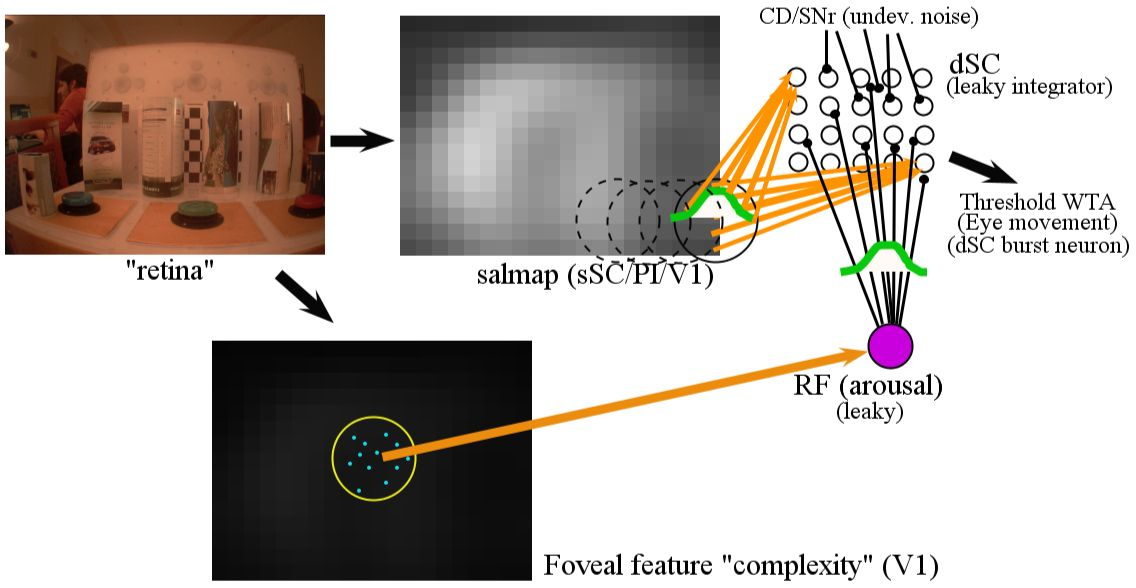
\includegraphics[width=15.0cm]{looking_prototype_model.jpg}
\caption{Graphical overview of connectivity and regions of network,
  and the general function of each region. Full-model anatomical
  correlates listed next to regions.}
\label{fig:looking_prototype_model}
\end{figure}

The network is made up of several main pieces
(Figure~\ref{fig:looking_prototype_model}). The overall theory of its
functionality is illustrated in
Figure~\ref{fig:looking_functional_loop}.

\subsection{Saliency Map}
Images (frames) come in (actually, one from each eye, left and right)
and are put through a saliency map (\cite{itti_etal_1998}), which
assigns a salience value to each location in the image by looking for
areas of high global ``uniqueness'' at many spatial scales. This is
accomplished by applying filters at many scales in parallel to detect
feature channels such as motion, color, intensity, orientation, etc,
and then subtracting and subsampling between sequential spatial
scales, within channels. This is meant to represent some sort of
``fast scene processing'' salience, which does not care so much about
the content at visual locations so much as the ``salience'' of
locations especially in relation to the rest of the visual field. It
is imagined that this type of saliency map would be used in orienting
behavior, which is of course exactly what the looking behavior in this
paper is about. Some of the saliency channels (color, orientation) are
not ones that would be processed by the superficial layers of the
superior colliculus (SC)(mostly responds to movement), nor is there
evidence for (explicit) spatial scales even in V1, so it is not clear
where a salience map would actually be implemented, especially in an
infant.

\subsection{Superior Colliculus - deep (integration, eye control)}
The instantaneous salience map calculated for every frame is treated
as ``input'' into a longer-term map made up of leaky integrating
neurons (non-firing). This is considered to correspond to the
intermediate/deep layers of SC, especially since this is the last
``stop'' before eye movements in our model. Each neurons membrane
potential $V_m$ is described by the equation:
\begin{equation}
\frac{\partial V_m}{\partial t} = \frac{-(V_m - V_{rest}) + R_m \cdot
  (I_{bg} + I_{syn})}{\tau_m}
\end{equation}
where $R_m$ is the membrane resistance (uniformly 1.0 M$\Omega$ for
all neurons), $I_{bg}$ the background current (uniformly 0.0 mV for
all neurons) and $I_{syn}$ the total current impinging from afferent
synapses. The $-V_m$ represents the leakage term, causing the membrane
potential to decay exponentially with time constant $\tau_m$
(uniformly 30 ms for all neurons, though since update was per-frame
this has no relation to real-time). The resting potential of the
membrane $V_{rest}$ is assumed to be 0 mV.

Afferent input into a dSC neuron from the instantaneous saliency map
is simply linearly summed into $I_{syn}$, after being multiplied by
the efficacy of the synapse connecting it. The synaptic weights and
connections are built initially using a 2-dimensional gaussian, with
standard deviation $\omega_w$ (1.5 for the experiments) and a cutoff
value (i.e. minimum weight outside of which region there are no
connections) $\chi$ (0.05 for experiments). This has the effect of
slightly blurring (low-pass-filtering) the instantaneous salmap (thus
bringing out ``masses'' of high salience more than just isolated
pixels of high salience). It also mimics the increase in receptive
field size one sees when moving more towards the dSC (many
pre-synaptic neurons connect to fewer post-synaptic neurons, in
retinotopically defined areas).

\subsection{Reticular Formation (arousal response to complexity)}
%HR deceleration, Richards etc.

Physiological functions (arousal, measured by heart rate) have been
shown to be correlated with attentional phases in infants
\cite{richards_casey_1990}. Some have hypothesized the underlying
circuits for these include e.g. the reticular formation (RF) which is
responsible for the ascending transport of neuromodulators (horomones)
to diverse regions of the brain. Such areas could become more active
in response to stimulating environments (i.e. with more complex
stimuli, more variation, etc.) and are also responsible for the lack
of responsiveness of infants without sufficient stimulation. Though,
endogenous ebb and flow guide a large part of the very young infant's
arousal/attentional state at any time.

The complexity-responsive functionality of the RF circuits are used as
a mechanism for determining (soft) looking time towards an
object. Really, it could be implemented via other things such as
simply probabilistic microsaccades that are more likely to get
``caught'' in the more complex stimulus. Since usually the amount of
looking time towards a stimulus during e.g. habituation experiments is
postulated to be a function of ``encoding'' of the stimulus (and thus,
longer for more complex stimuli), yet we have explicitly lesioned
those areas that are ``making progress'' in any sense (or learning),
there must be some other mechanism than simply ``learning'' that
drives looking time towards stimuli. Since in habituation experiments
the salience etc. of stimuli is controlled, it is not easy to decouple
the habituation response from the ``baseline'' stimulus response. Note
also that more complex mechanisms, e.g. encoding into some sort of
short-term memory, waiting for a non-transient response/cycle of some
minimal error threshold in response to the stimulus, could be how this
stimulus complexity causes longer looking times, but the current
mechanism at least attempts to capture the phenomenon if not the
mechanism. This is perhaps one of the least understood areas of
oculomotor behavior -- namely, in absense of any scene change, what
causes the infant to look away? Several observations exist that
correlate with the phenomenon, e.g. the dying out of fixation neurons
in dSC, changes in activity in SNr, CD, and the buildup of burst
neurons in dSC, but the real dynamics and mechanisms and how all these
work together to move attention (fixation) are not well
understood. This is one of the things this model and the more
plausible one hope to offer explanations for.

In the model the RF is modeled as a single leaky neuron. One can think
of it as population coding of the activity of some region that got a
shot of neuromodulator/horomone cocktail in response to exciting
foveal stimuli. The RF neuron inhibits every region of the dSC, so
that more activation of the RF will result in more inhibition of SC
(pushing the neurons there to very negative potentials), and thus it
will take longer for SC neurons to recover via the normal continuous
input coming from e.g. the instantaneous saliency map and the gaussian
noise from SNr. However, to prevent the continuous fixation over
multiple ``refixations'' of the central area (which might not be coded
in mammals, i.e. we wouldn't have to worry about the currently
foveated area ever getting burst neurons activated since there are no
corresponding burst neurons there) the weighting of this inhibitory
projection is topologically modulated, such that more foveal/central
positions have stronger inhibitory weights than the periphery (which
still have some baseline inhibitory weight).

Thus, the weight of a point in the retinotopic projection as a
function of distance from the centre of the fovea is equal to the
value at that point of a gaussian centred on the centre, with
amplitude $\alpha$ (6.0), variance $\sigma$ (1.5), and baseline
(i.e. y-shift) $\beta$ (1.0).

When a gaze shift is made, the ``complexity'' $c_f$ of the current
foveal content is scaled and injected into the RF neuron (the RF
neuron's $V_m$ is set to $c_f$. In this case, as a standing, the
complexity is calculated as the number of Harris feature points
(thresholded 1-d gaussians LPFs run along the x- and y-dimensions)
within a radius $r$ of the centre of the image. In binocular cases the
two eyes are simply summed together linearly.

The RF neuron's membrane potential ($V_{RF}$) decays exponentially
with some time constant $\tau_{RF}$ (500ms, though again since in the
experiments update of the saliency model is not locked to real time
the units are arbitrary w.r.t. the experiments), i.e.
\begin{equation}
\frac{\partial V_{RF}}{\partial t} = \frac{-V_{RF}}{\tau_m}
\end{equation}

The membrane potential of RF is injected directly into all (e.g. dSC)
post-synaptic neurons, simply linearly scaled by the weight of the
synapse connecting RF with that neuron.

\subsection{Substantia Nigra pars reticulata (Gaussian noise)}
%because of e.g. unstable dynamics from dopamine...SNc...

Caudate Nucleus (CD) and SNr neurons show visual and habituation
responses \cite{hikosaka_wurtz_1983_SNr1}, which implies they are at
play in normal visual search behavior and/or habituation
learning. Assuming it's just habituation or even considering they are
engaged in disgengagement and thus normal visual looking behavior
(\cite{johnson_1990}), these disengagement and habituation behaviors
are not seen in infants or in limbic-cortex lesioned primates,
respectively. This suggests that the SNr itself, it's afferents, or
its efferents to dSC are undeveloped in the young infants. SNr-dSC
projections are known to be strongly GABAergic and thus inhibitory,
and to receive inhibitory projections from CD (``dis-inhibitory'',
which in turns gets input from a variety of regions as well as having
interesting intrinsic dynamics involving dopamine via SNc). We model
these dynamics and the product of immaturity by simply considering the
baseline of SC as already receiving some amount of inhibition from the
tonically firing SNr GABAergic neurons, and then add or sutract
gaussian noise (gaussian random variables) from the synaptic input to
each dSC neuron on every time step. The probability of drawing an
input of strength of $\delta$ is probabilistically based on the mass
of the gaussian at the point, thus small numbers are likely, and very
far out numbers are less likely. In the experiments, the noise is
drawn from a gaussian with $\sigma$ of 0.01 and amplitude (scale of
output inputs) of 1.0.

%2) OVERALL FUNCTIONALITY (i.e. rationale/mechanism of functioning to achieve desired behavior)
\begin{figure} [!t]
\centering
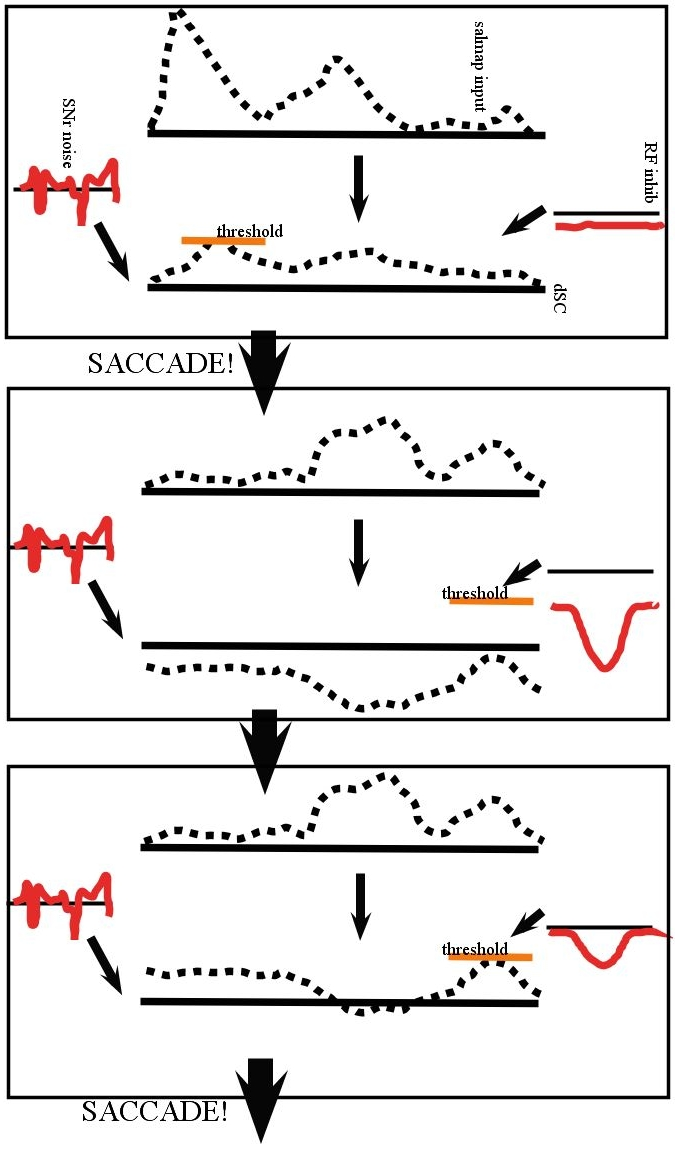
\includegraphics[width=15.0cm]{looking_functional_loop.jpg}
\caption{Intended loop dynamics of the model through several
  fixation-saccade iterations. Intended local circuit response
  properties listed where predictable.}
\label{fig:looking_functional_loop}
\end{figure}


\section{Method and Results}
The prototype model was implemented on an iCub robot
(Figure~\ref{fig:icub_head}). It has two pan-tilt-vergence eyes
mounted in a head supported by a yaw-pitch-twist neck (see
picture). Eye movements were accomplished by way of a vergence-control
mechanism which ran in a closed-loop fashion with visual input (this
was not realistic, but necessary because of limited time and a lack of
familiarity with the iCub and with binocular systems. It is not clear
how the problem of vergence is solved in infants but it is clear that
saccades are not closed loop or vision-driven but are ballistic and
motor-driven~\cite{hainline_1998}). Since the model was turned off
during ``saccades'' this had no effect on the collected data, though
from a real-time point of view it was very slow compared with actual
saccades (limitations of the motors). Coordinated movement of the head
and eyes is likewise probably unrealistic in such young infants. The
more complete model will need to account for eye movements while
either avoiding or solving these non-trivial problems.

%PICTURE icub
\begin{figure} [!t]
\centering
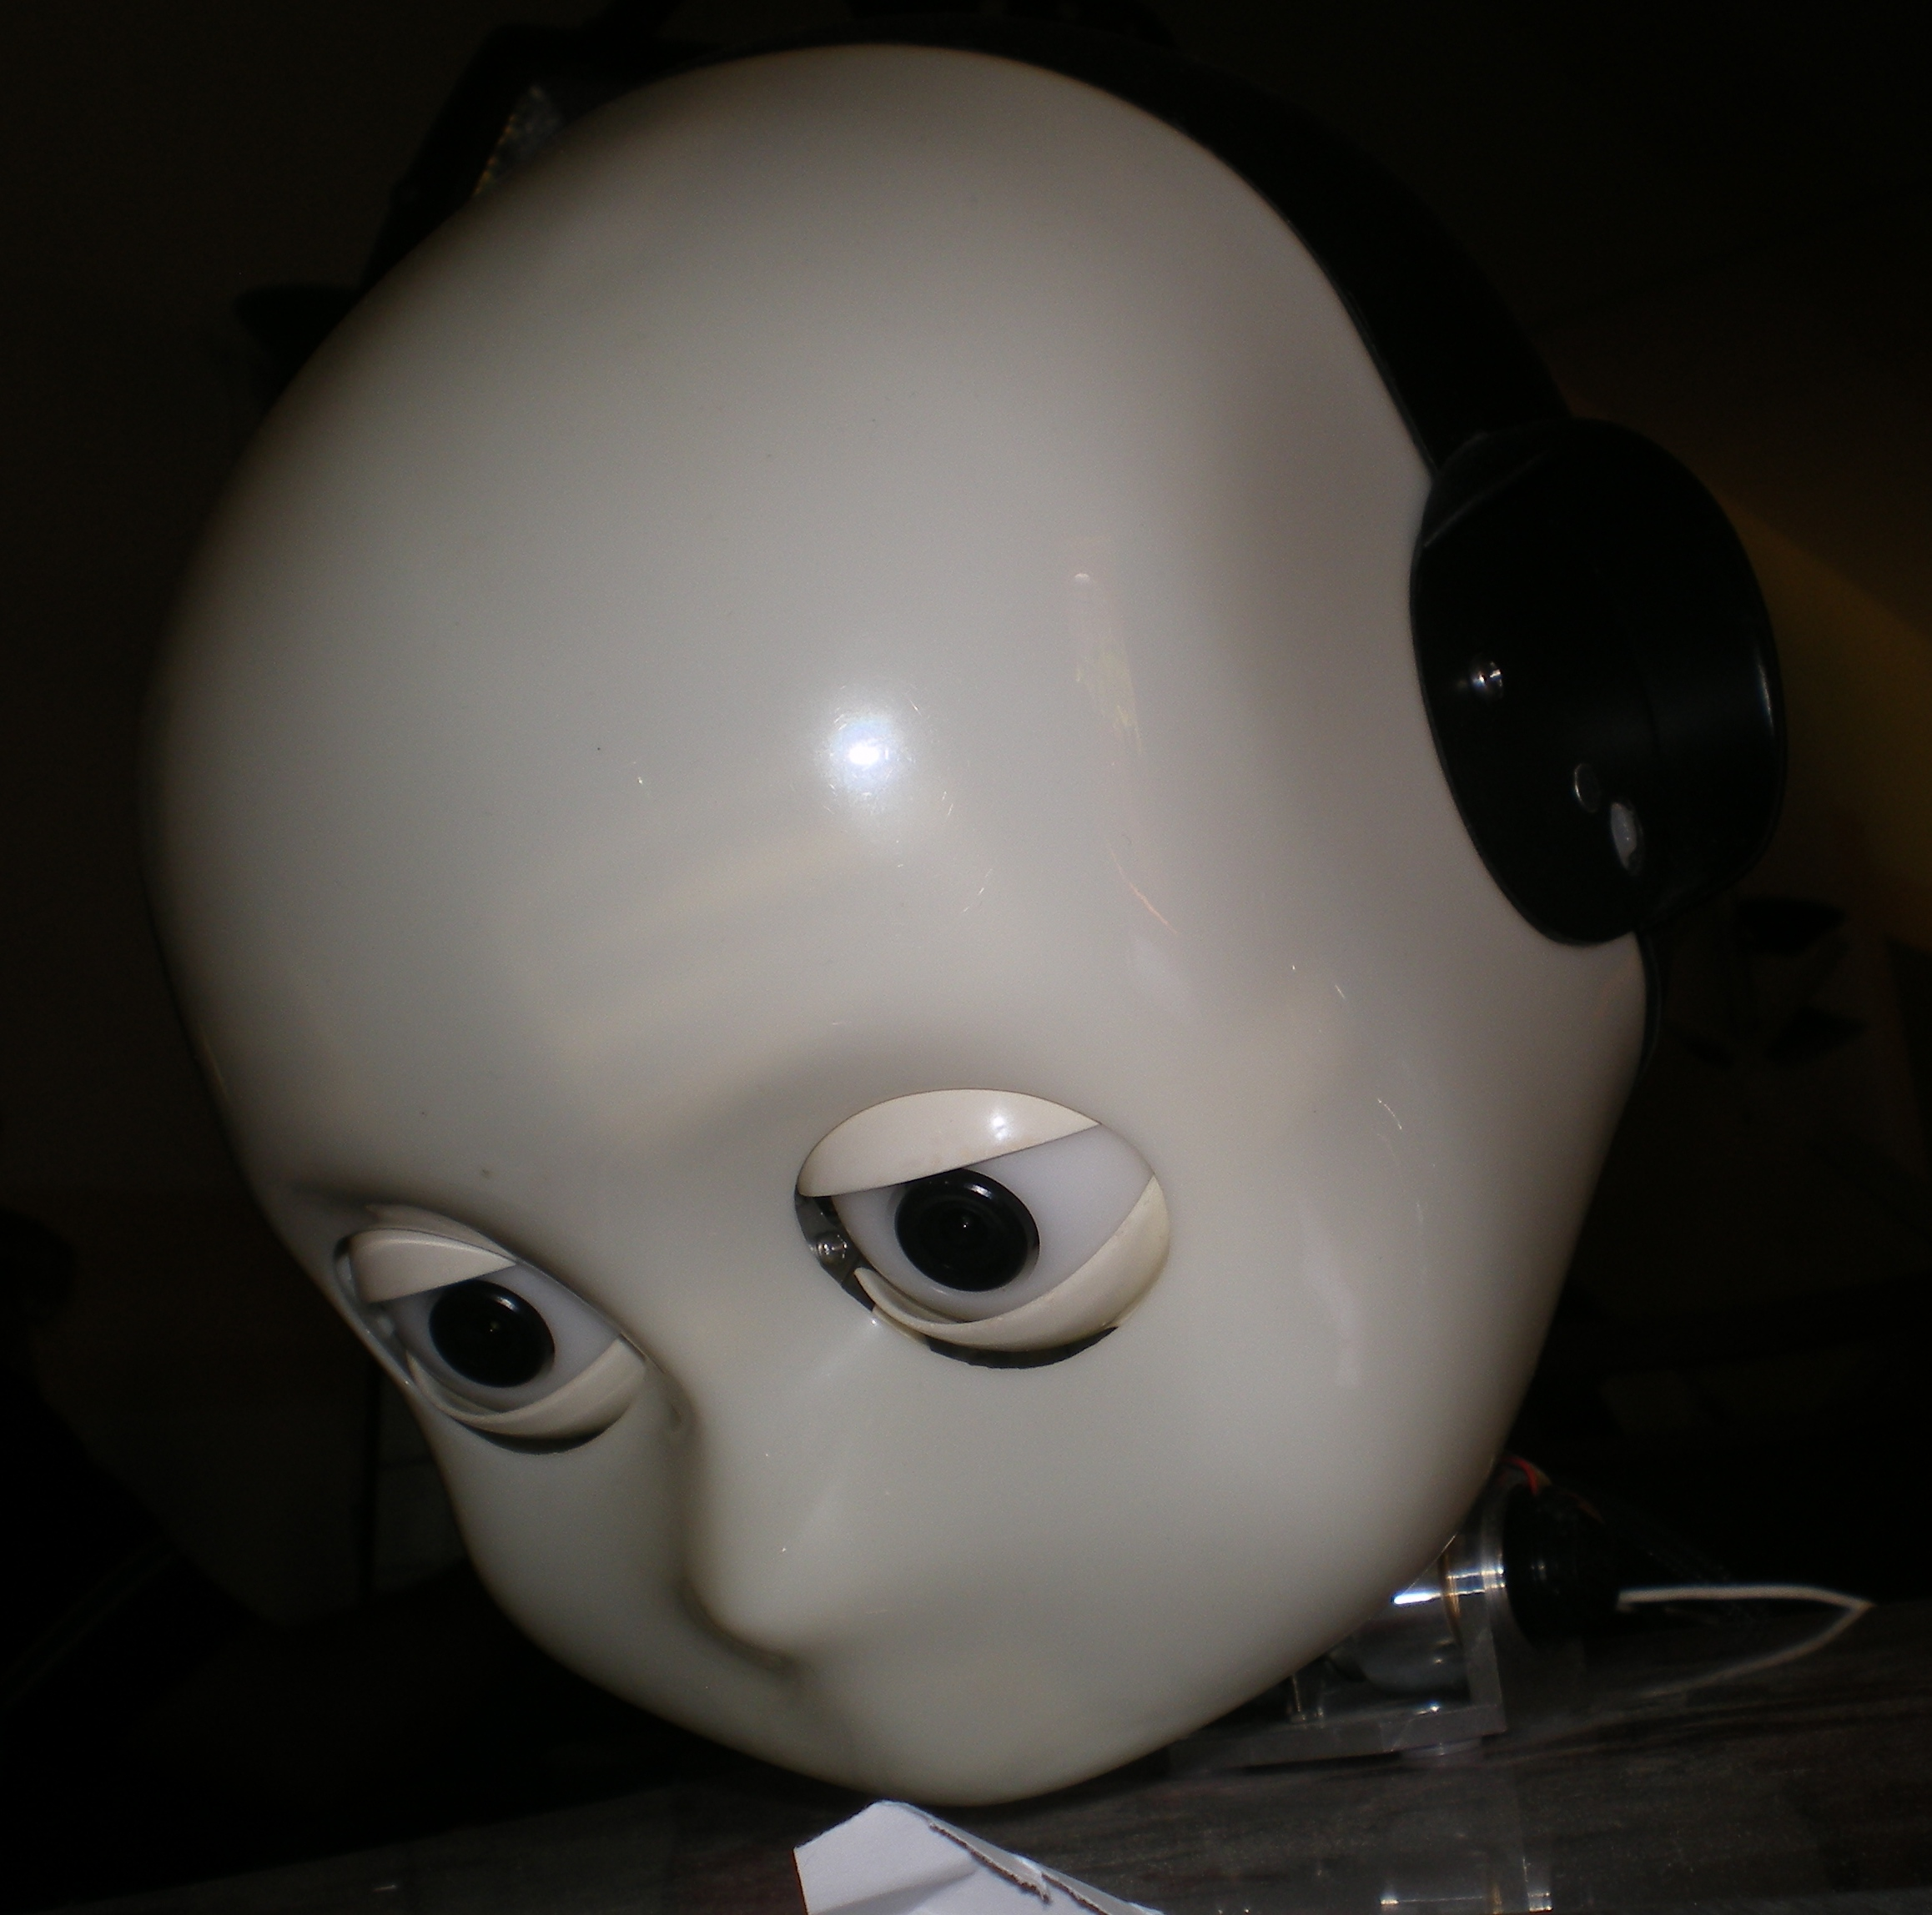
\includegraphics[width=5.0cm]{icub_head.jpg}
\caption{The iCub head that was used for the experiments.}
\label{fig:icub_head}
\end{figure}

The robot instantiated the network and was placed in front of a scene.
The amount of time spent looking at objects and the ``complexity'' of
the object was recorded. The trajectory (i.e. ordering) of looking
among the objects was recorded.

%PICTURE exp setup (example environ) also mention movement type thing?
%PICTURE icub
\begin{figure} [!t]
\centering
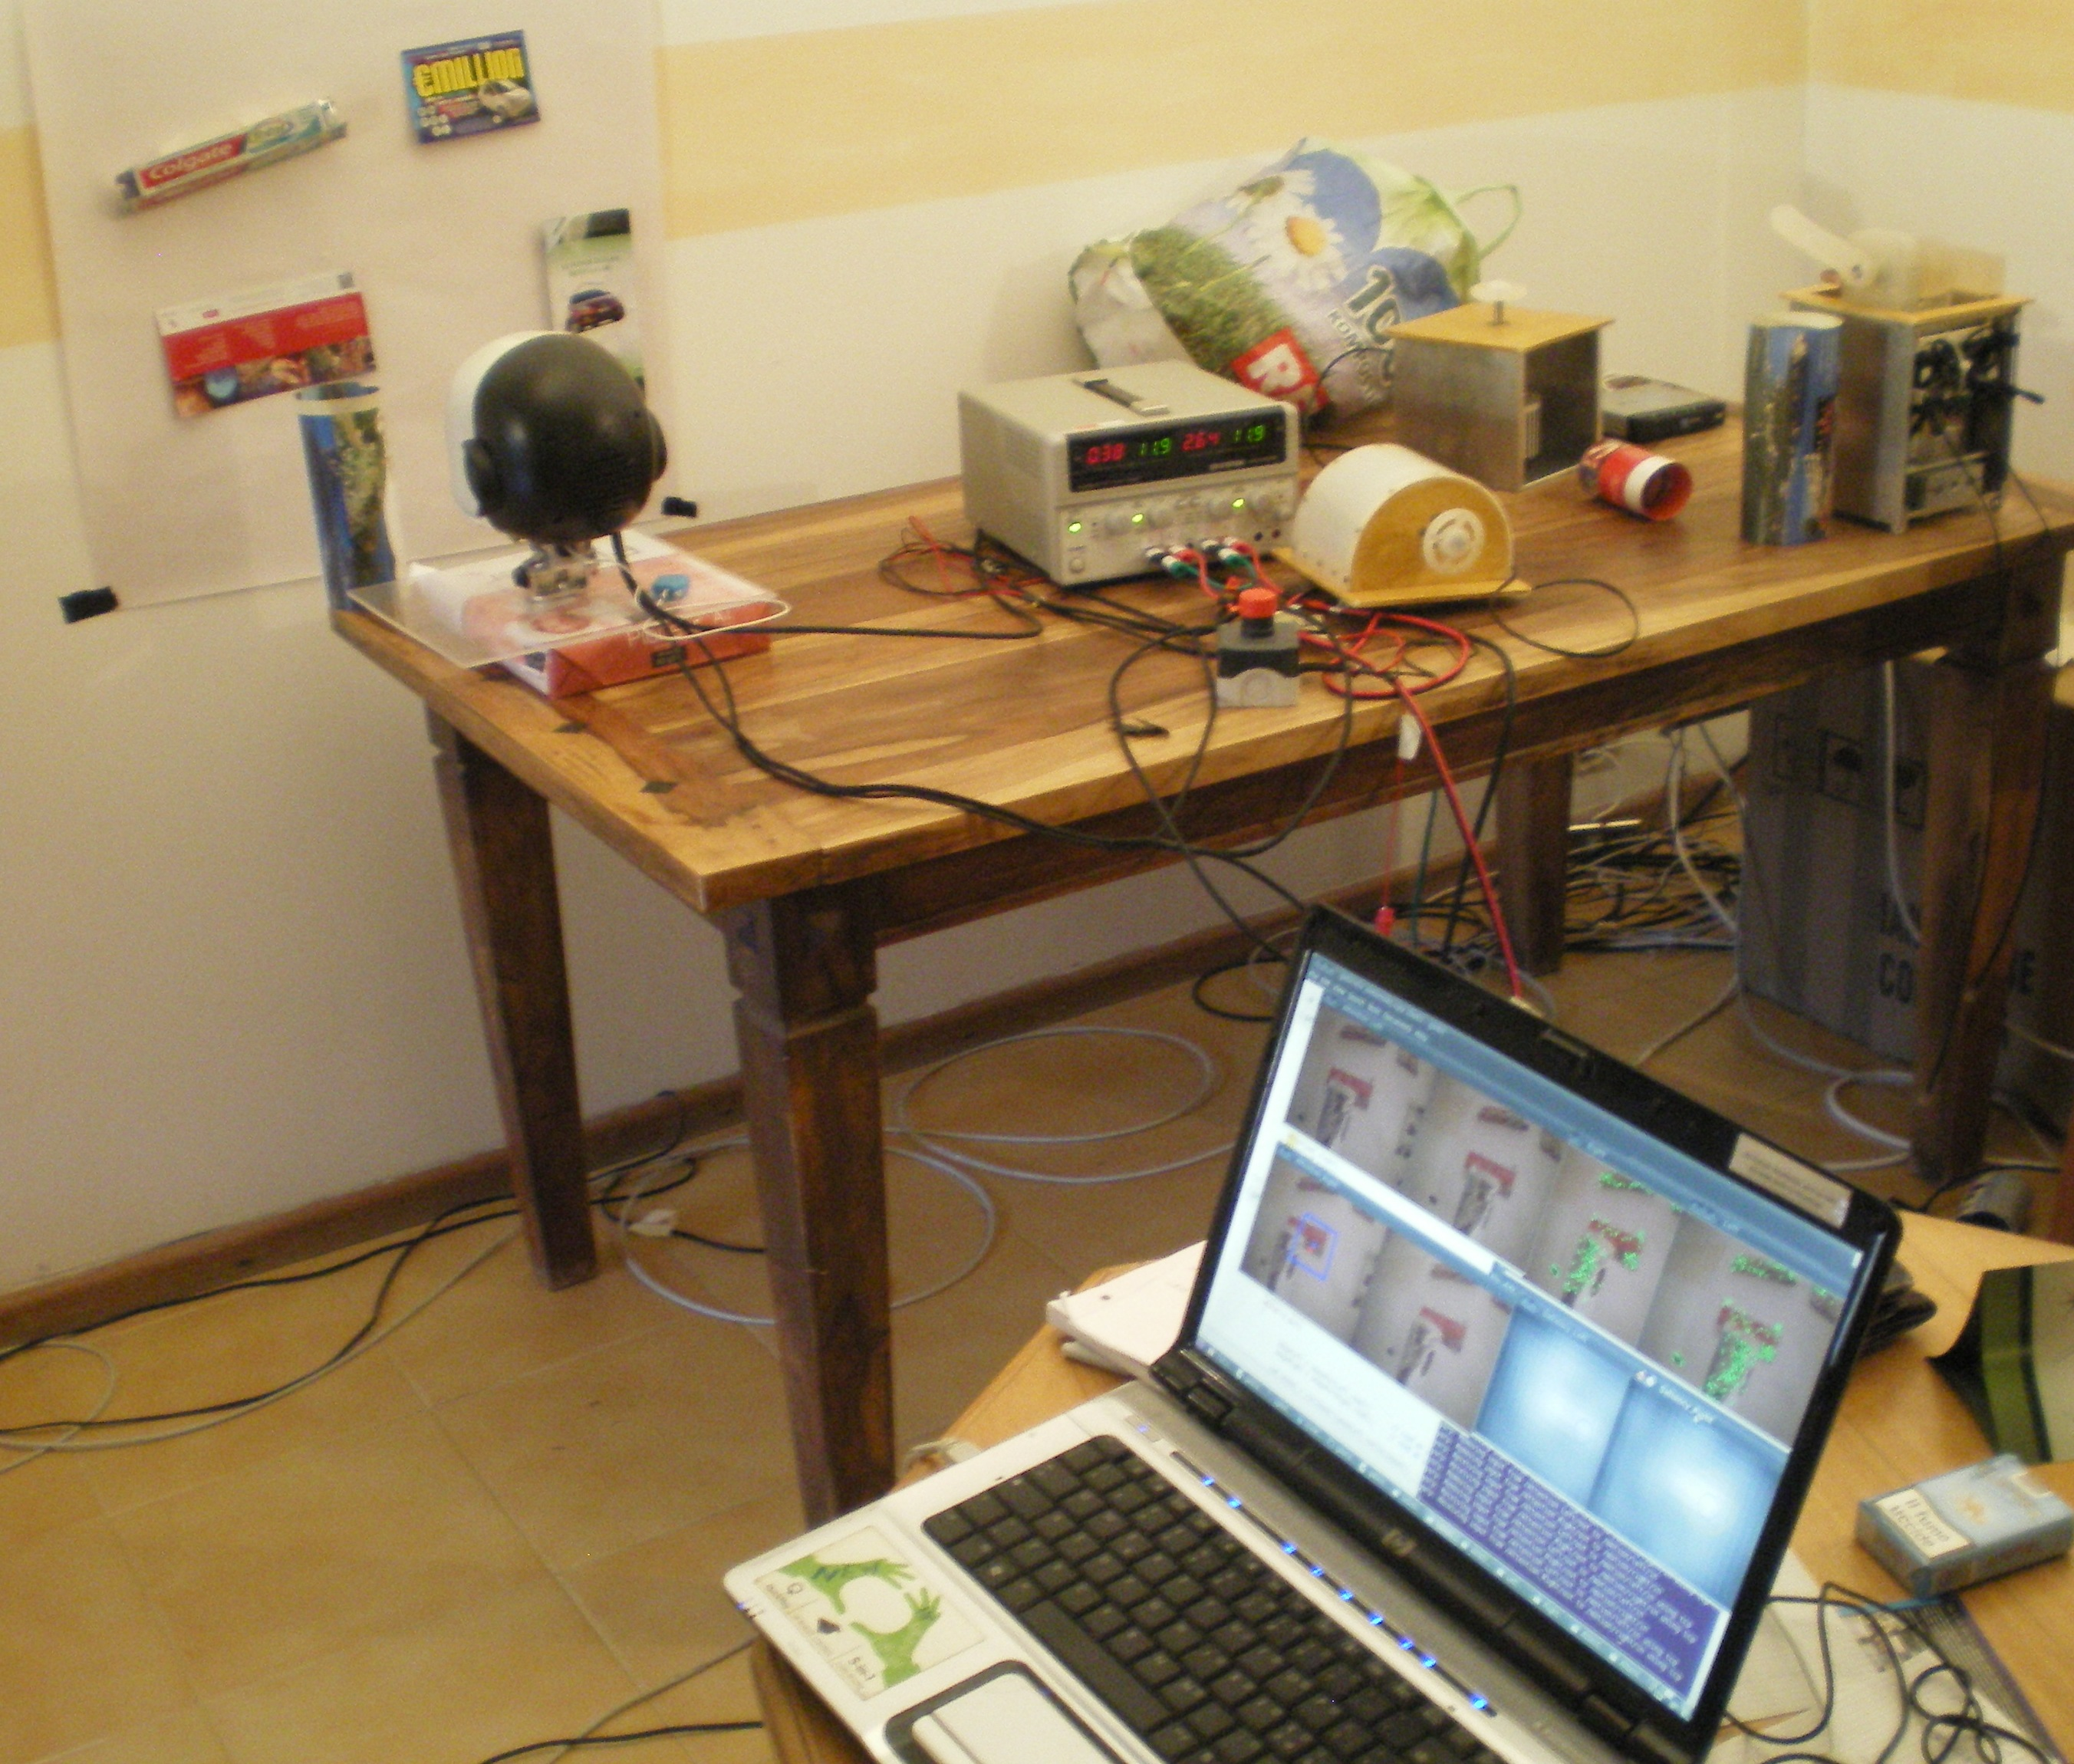
\includegraphics[width=7.0cm]{icub_setup.jpg}
\caption{A picture of the experimental setup that was used during the
  experiments. The type of environment presented can be seen in front
  of the iCub head in the upper-left corner.}
\label{fig:icub_setup}
\end{figure}

%********************RESULTS******************%
\subsection{Results}
Results will go here... Based on runs on single frames (see
testonppm.cpp) the decaying-inhibition dynamics of the model work as
intended. To demonstrate this, see
Figure~\ref{fig:complex_vs_fixtime}, plotting the results of automated
experiments with the model measuring the time between first fixation
and second fixation as a function of the complexity of the foveal
image (x-axis).
\begin{figure} [!t]
\centering
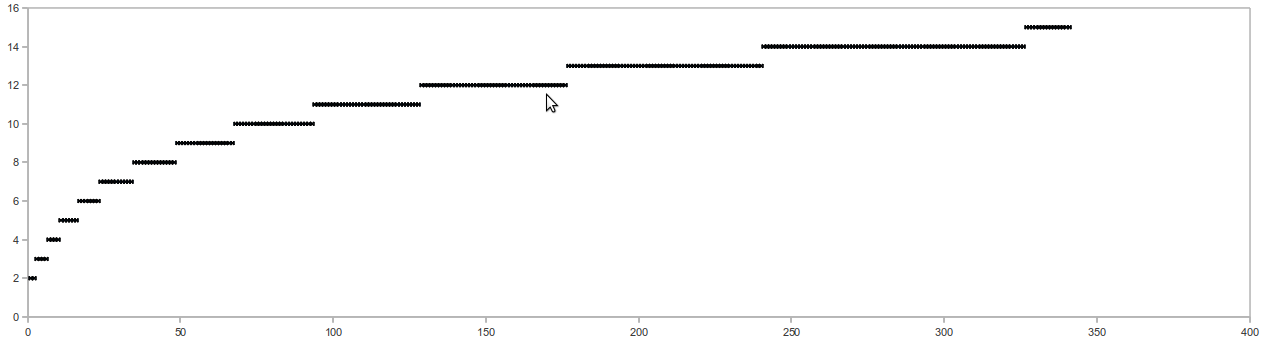
\includegraphics[width=15.0cm]{complex_vs_fixtime.png}
\caption{Plot of the time between fixations (i.e. fixation time to
  that foveal region) for varying levels of foveal complexity (the
  manipulated variable in these experiments). Note the logarithmic
  pattern that emerges: for very low complexities, fixation is
  disengaged quickly, and for slightly different complexities the
  looking time differs, but as complexity increases, the looking time
  saturates to a maximum.}
\label{fig:complex_vs_fixtime}
\end{figure}

This is the desired behavior, and would result in (at least) fixation
times that follow the desired model of fixation time. For the
longer-term looking dynamics, however, since foveation of the salient
stimulus is assumed, it's impossible to test the looking dynamics
without running on the robot or in a simulation environment that moves
the visual field.

\section{Conclusion}
By design, the mechanism to determine looking time towards a foveal
stimulus as a function of its complexity was successful, but this is
not the interesting result since these dynamics are predicted and
necessitated by the simple mechanism.

The interesting bit will be the inter-object looking behavior in a
real environment. Will, and how often will, the system make saccades
to ``noise'' areas but then quickly look away because of lack of
complexity?

In the future, the model will be implemented as the more complex
anatomical circuit, the saliency map replaced with proper neural code
from the eye-up, and the actual neurons ``fudged'' in most of the
areas and their dynamics actually simulated. The benefit of building
the more realistic model will be to actually look at the different
dynamics of the model in reaction to the changing environment, since
that kind of interaction can not be easily predicted or simulated.

\bibliographystyle{apacite} \bibliography{bib}

\end{document}
